\documentclass{article}\usepackage[]{graphicx}\usepackage[]{xcolor}
% maxwidth is the original width if it is less than linewidth
% otherwise use linewidth (to make sure the graphics do not exceed the margin)
\makeatletter
\def\maxwidth{ %
  \ifdim\Gin@nat@width>\linewidth
    \linewidth
  \else
    \Gin@nat@width
  \fi
}
\makeatother

\definecolor{fgcolor}{rgb}{0.345, 0.345, 0.345}
\newcommand{\hlnum}[1]{\textcolor[rgb]{0.686,0.059,0.569}{#1}}%
\newcommand{\hlsng}[1]{\textcolor[rgb]{0.192,0.494,0.8}{#1}}%
\newcommand{\hlcom}[1]{\textcolor[rgb]{0.678,0.584,0.686}{\textit{#1}}}%
\newcommand{\hlopt}[1]{\textcolor[rgb]{0,0,0}{#1}}%
\newcommand{\hldef}[1]{\textcolor[rgb]{0.345,0.345,0.345}{#1}}%
\newcommand{\hlkwa}[1]{\textcolor[rgb]{0.161,0.373,0.58}{\textbf{#1}}}%
\newcommand{\hlkwb}[1]{\textcolor[rgb]{0.69,0.353,0.396}{#1}}%
\newcommand{\hlkwc}[1]{\textcolor[rgb]{0.333,0.667,0.333}{#1}}%
\newcommand{\hlkwd}[1]{\textcolor[rgb]{0.737,0.353,0.396}{\textbf{#1}}}%
\let\hlipl\hlkwb

\usepackage{framed}
\makeatletter
\newenvironment{kframe}{%
 \def\at@end@of@kframe{}%
 \ifinner\ifhmode%
  \def\at@end@of@kframe{\end{minipage}}%
  \begin{minipage}{\columnwidth}%
 \fi\fi%
 \def\FrameCommand##1{\hskip\@totalleftmargin \hskip-\fboxsep
 \colorbox{shadecolor}{##1}\hskip-\fboxsep
     % There is no \\@totalrightmargin, so:
     \hskip-\linewidth \hskip-\@totalleftmargin \hskip\columnwidth}%
 \MakeFramed {\advance\hsize-\width
   \@totalleftmargin\z@ \linewidth\hsize
   \@setminipage}}%
 {\par\unskip\endMakeFramed%
 \at@end@of@kframe}
\makeatother

\definecolor{shadecolor}{rgb}{.97, .97, .97}
\definecolor{messagecolor}{rgb}{0, 0, 0}
\definecolor{warningcolor}{rgb}{1, 0, 1}
\definecolor{errorcolor}{rgb}{1, 0, 0}
\newenvironment{knitrout}{}{} % an empty environment to be redefined in TeX

\usepackage{alltt}
\usepackage[margin=1.0in]{geometry} % To set margins
\usepackage{amsmath}  % This allows me to use the align functionality.
                      % If you find yourself trying to replicate
                      % something you found online, ensure you're
                      % loading the necessary packages!
\usepackage{amsfonts} % Math font
\usepackage{fancyvrb}
\usepackage{hyperref} % For including hyperlinks
\usepackage[shortlabels]{enumitem}% For enumerated lists with labels specified
                                  % We had to run tlmgr_install("enumitem") in R
\usepackage{float}    % For telling R where to put a table/figure
\usepackage{natbib}        %For the bibliography
\bibliographystyle{apalike}%For the bibliography
\IfFileExists{upquote.sty}{\usepackage{upquote}}{}
\begin{document}


\cite{Kasdin25} show that dopamine in the brains of young zebra finches acts as 
a learning signal, increasing when they sing closer to their adult song and 
decreasing when they sing further away, effectively guiding their vocal 
development through trial-and-error. This suggests that complex natural 
behaviors, like learning to sing, are shaped by dopamine-driven reinforcement 
learning, similar to how artificial intelligence learns. You can find the 
paper at this link:
\href{https://www.nature.com/articles/s41586-025-08729-1}{{https://www.nature.com/articles/s41586-025-08729-1}.}.

Note they measure dopamine using fibre photometry, changes in the fluorescence
indicate dopamine changes in realtime. Their specific measurement considers 
changes in flourescence in 100-ms windows between 200 and 300 ms from the start 
of singing, averaged across development.

\begin{enumerate}
%%%%%%%%%%%%%%%%%%%%%%%%%%%%%%%%%%%%%%%%%%%%%%%%%%%%%%%%%%%%%%%%%
% CONDUCT A POWER ANALYSIS
%%%%%%%%%%%%%%%%%%%%%%%%%%%%%%%%%%%%%%%%%%%%%%%%%%%%%%%%%%%%%%%%%
\item Using the \texttt{pwr} package for \texttt{R} \citep{pwr},
conduct a power analysis. How many observations would the researchers 
need to detect a moderate-to-large effect ($d=0.65$) when using 
$\alpha=0.05$ and default power (0.80) for a two-sided one sample 
$t$ test.
\begin{knitrout}
\definecolor{shadecolor}{rgb}{0.969, 0.969, 0.969}\color{fgcolor}\begin{kframe}
\begin{alltt}
\hlkwd{library}\hldef{(pwr)}
\hldef{power.analysis} \hlkwb{=} \hlkwd{pwr.t.test}\hldef{(}\hlkwc{d}\hldef{=}\hlnum{0.65}\hldef{,}
                            \hlkwc{sig.level} \hldef{=} \hlnum{0.05}\hldef{,}
                            \hlkwc{power} \hldef{=} \hlnum{0.80}\hldef{,}
                            \hlkwc{type} \hldef{=} \hlsng{"one.sample"}\hldef{,}
                            \hlkwc{alternative} \hldef{=} \hlsng{"two.sided"}\hldef{)}
\end{alltt}
\end{kframe}
\end{knitrout}
I got that n = 20.58039, so 21 observations are required in order to detect a moderate-to-large effect when using this significance level and power.
%%%%%%%%%%%%%%%%%%%%%%%%%%%%%%%%%%%%%%%%%%%%%%%%%%%%%%%%%%%%%%%%%
% COLLECT DATA
%%%%%%%%%%%%%%%%%%%%%%%%%%%%%%%%%%%%%%%%%%%%%%%%%%%%%%%%%%%%%%%%%
\item Click the link to go to the paper. Find the source data for 
Figure 2. Download the Excel file. Describe what you needed to
do to collect the data for Figure 2(g). Note that you only need the 
\texttt{closer\_vals} and \texttt{further\_vals}. Ensure to 
\texttt{mutate()} the data to get a difference 
(e.g., \texttt{closer\_vals - further\_vals}).
\begin{knitrout}
\definecolor{shadecolor}{rgb}{0.969, 0.969, 0.969}\color{fgcolor}\begin{kframe}
\begin{alltt}
\hlkwd{library}\hldef{(tidyverse)}
\hldef{dopamine.data} \hlkwb{=} \hlkwd{read_csv}\hldef{(}\hlsng{"DopamineData.csv"}\hldef{)}
\hldef{dopamine.data} \hlkwb{=} \hldef{dopamine.data |>}
  \hlcom{#create column that contains the difference between farther and closer values}
  \hlkwd{mutate}\hldef{(}\hlkwc{difference} \hldef{= Closer_vals} \hlopt{-} \hldef{Farther_vals)}
\end{alltt}
\end{kframe}
\end{knitrout}
To collect the data for Figure 2(g), I had to first download the entire source data file for all of Figure 2. Then, I extracted the data from the Farther\textunderscore vals and Closer\textunderscore vals tabs which correspond to Figure 2(g). Lastly, I put the columns side-by-side into a new Excel file, and downloaded it as a .csv file.
%%%%%%%%%%%%%%%%%%%%%%%%%%%%%%%%%%%%%%%%%%%%%%%%%%%%%%%%%%%%%%%%%
% SUMMARIZE DATA
%%%%%%%%%%%%%%%%%%%%%%%%%%%%%%%%%%%%%%%%%%%%%%%%%%%%%%%%%%%%%%%%%
\item Summarize the data.
\begin{enumerate}
  \item Summarize the further data. Do the data suggest that
   dopamine in the brains of young zebra finches decreases when
   they sing further away?
   \item Summarize the closer data. Do the data suggest that
   dopamine in the brains of young zebra finches increases when
   they sing closer to their adult song?
  \item Summarize the paired differences. Do the data suggest
  that there is a difference between dopamine in the brains of
  young zebra finches when they sing further away compared to 
  closer to their adult song?
  
\begin{table}[H]
\centering
\begin{tabular}{rrrrrr} 
  \hline
 & min & max & median & mean & sd \\
  \hline
farther & -0.60 & -0.03 & -0.19 & -0.20 & 0.13 \\
  closer & 0.00 & 0.34 & 0.15 & 0.16 & 0.09 \\
  differences & 0.04 & 0.93 & 0.33 & 0.36 & 0.21 \\
    \hline
\end{tabular}
\caption{Numerical Summary for the further, closer, and differences data}
\label{table:reference}
\end{table}
\begin{knitrout}
\definecolor{shadecolor}{rgb}{0.969, 0.969, 0.969}\color{fgcolor}\begin{kframe}
\begin{alltt}
\hlkwd{library}\hldef{(patchwork)}
\hldef{summary} \hlkwb{=} \hlkwa{function}\hldef{(}\hlkwc{data}\hldef{) \{}
  \hldef{mean} \hlkwb{=} \hlkwd{mean}\hldef{(data)}
  \hldef{min} \hlkwb{=} \hlkwd{min}\hldef{(data)}
  \hldef{max} \hlkwb{=} \hlkwd{max}\hldef{(data)}
  \hldef{sd} \hlkwb{=} \hlkwd{sd}\hldef{(data)}
  \hldef{median} \hlkwb{=} \hlkwd{median}\hldef{(data)}
  \hlkwd{return}\hldef{(}\hlkwd{c}\hldef{(min, max, median, mean, sd))}
\hldef{\}}
\hldef{farther} \hlkwb{=} \hlkwd{summary}\hldef{(dopamine.data}\hlopt{$}\hldef{`Farther_vals`)}
\hldef{closer} \hlkwb{=} \hlkwd{summary}\hldef{(dopamine.data}\hlopt{$}\hldef{`Closer_vals`)}
\hldef{differences} \hlkwb{=} \hlkwd{summary}\hldef{(dopamine.data}\hlopt{$}\hldef{difference)}

\hldef{table} \hlkwb{=} \hlkwd{data.frame}\hldef{()}
\hldef{table} \hlkwb{=} \hlkwd{rbind}\hldef{(farther,}
              \hldef{closer,}
              \hldef{differences) |>} \hlkwd{as.data.frame}\hldef{()}
\hldef{summary.table} \hlkwb{=} \hldef{table |>}
  \hlkwd{rename}\hldef{(}\hlkwc{min} \hldef{=} \hlsng{"V1"}\hldef{,}
         \hlkwc{max} \hldef{=} \hlsng{"V2"}\hldef{,}
         \hlkwc{median} \hldef{=} \hlsng{"V3"}\hldef{,}
         \hlkwc{mean} \hldef{=} \hlsng{"V4"}\hldef{,}
         \hlkwc{sd} \hldef{=} \hlsng{"V5"}\hldef{)}

\hldef{farther.plot} \hlkwb{=} \hlkwd{ggplot}\hldef{(}\hlkwc{data} \hldef{= dopamine.data,} \hlkwd{aes}\hldef{(}\hlkwc{x}\hldef{=`Farther_vals`))}\hlopt{+}
  \hlkwd{geom_histogram}\hldef{(}\hlkwd{aes}\hldef{(}\hlkwc{y}\hldef{=}\hlkwd{after_stat}\hldef{(density)),}
                 \hlkwc{breaks}\hldef{=}\hlkwd{seq}\hldef{(}\hlopt{-}\hlnum{0.7}\hldef{,}\hlnum{0}\hldef{,}\hlnum{0.07}\hldef{))} \hlopt{+}
  \hlkwd{geom_hline}\hldef{(}\hlkwc{yintercept}\hldef{=}\hlnum{0}\hldef{)}\hlopt{+}
  \hlkwd{theme_bw}\hldef{()}\hlopt{+}
  \hlkwd{geom_density}\hldef{(}\hlkwc{color} \hldef{=} \hlsng{"blue"}\hldef{)} \hlopt{+}
  \hlkwd{xlab}\hldef{(}\hlsng{"Change in dopamine"}\hldef{)}\hlopt{+}
  \hlkwd{ylab}\hldef{(}\hlsng{"Density"}\hldef{)}\hlopt{+}
  \hlkwd{labs}\hldef{(}\hlkwc{color} \hldef{=} \hlsng{""}\hldef{,} \hlkwc{title} \hldef{=} \hlsng{"Change in dopamine levels when further away"}\hldef{)} \hlopt{+}
  \hlkwd{theme}\hldef{(}\hlkwc{plot.title} \hldef{=} \hlkwd{element_text}\hldef{(}\hlkwc{size} \hldef{=} \hlnum{10}\hldef{))}
\hldef{closer.plot} \hlkwb{=} \hlkwd{ggplot}\hldef{(}\hlkwc{data} \hldef{= dopamine.data,} \hlkwd{aes}\hldef{(}\hlkwc{x}\hldef{=`Closer_vals`))}\hlopt{+}
  \hlkwd{geom_histogram}\hldef{(}\hlkwd{aes}\hldef{(}\hlkwc{y}\hldef{=}\hlkwd{after_stat}\hldef{(density)),}
                 \hlkwc{breaks}\hldef{=}\hlkwd{seq}\hldef{(}\hlnum{0}\hldef{,}\hlnum{0.35}\hldef{,}\hlnum{0.035}\hldef{))} \hlopt{+}
  \hlkwd{geom_hline}\hldef{(}\hlkwc{yintercept}\hldef{=}\hlnum{0}\hldef{)}\hlopt{+}
  \hlkwd{theme_bw}\hldef{()}\hlopt{+}
  \hlkwd{geom_density}\hldef{(}\hlkwc{color} \hldef{=} \hlsng{"blue"}\hldef{)} \hlopt{+}
  \hlkwd{xlab}\hldef{(}\hlsng{"Change in dopamine"}\hldef{)}\hlopt{+}
  \hlkwd{ylab}\hldef{(}\hlsng{"Density"}\hldef{)}\hlopt{+}
  \hlkwd{labs}\hldef{(}\hlkwc{color} \hldef{=} \hlsng{""}\hldef{,} \hlkwc{title} \hldef{=} \hlsng{"Change in dopamine levels when closer"}\hldef{)} \hlopt{+}
  \hlkwd{theme}\hldef{(}\hlkwc{plot.title} \hldef{=} \hlkwd{element_text}\hldef{(}\hlkwc{size} \hldef{=} \hlnum{10}\hldef{))}
\hldef{differences.plot} \hlkwb{=} \hlkwd{ggplot}\hldef{(}\hlkwc{data} \hldef{= dopamine.data,} \hlkwd{aes}\hldef{(}\hlkwc{x}\hldef{=difference))}\hlopt{+}
  \hlkwd{geom_histogram}\hldef{(}\hlkwd{aes}\hldef{(}\hlkwc{y}\hldef{=}\hlkwd{after_stat}\hldef{(density)),}
                 \hlkwc{breaks}\hldef{=}\hlkwd{seq}\hldef{(}\hlnum{0}\hldef{,}\hlnum{1}\hldef{,}\hlnum{0.08}\hldef{))} \hlopt{+}
  \hlkwd{geom_hline}\hldef{(}\hlkwc{yintercept}\hldef{=}\hlnum{0}\hldef{)}\hlopt{+}
  \hlkwd{theme_bw}\hldef{()}\hlopt{+}
  \hlkwd{geom_density}\hldef{(}\hlkwc{color} \hldef{=} \hlsng{"blue"}\hldef{)} \hlopt{+}
  \hlkwd{xlab}\hldef{(}\hlsng{"Difference between changes in dopamine"}\hldef{)}\hlopt{+}
  \hlkwd{ylab}\hldef{(}\hlsng{"Density"}\hldef{)}\hlopt{+}
  \hlkwd{labs}\hldef{(}\hlkwc{title} \hldef{=} \hlsng{"Difference in dopamine levels when further away vs. closer"}\hldef{)} \hlopt{+}
  \hlkwd{theme}\hldef{(}\hlkwc{plot.title} \hldef{=} \hlkwd{element_text}\hldef{(}\hlkwc{size} \hldef{=} \hlnum{11}\hldef{))}
\hldef{(farther.plot} \hlopt{+} \hldef{closer.plot)} \hlopt{/} \hldef{differences.plot}
\end{alltt}
\end{kframe}
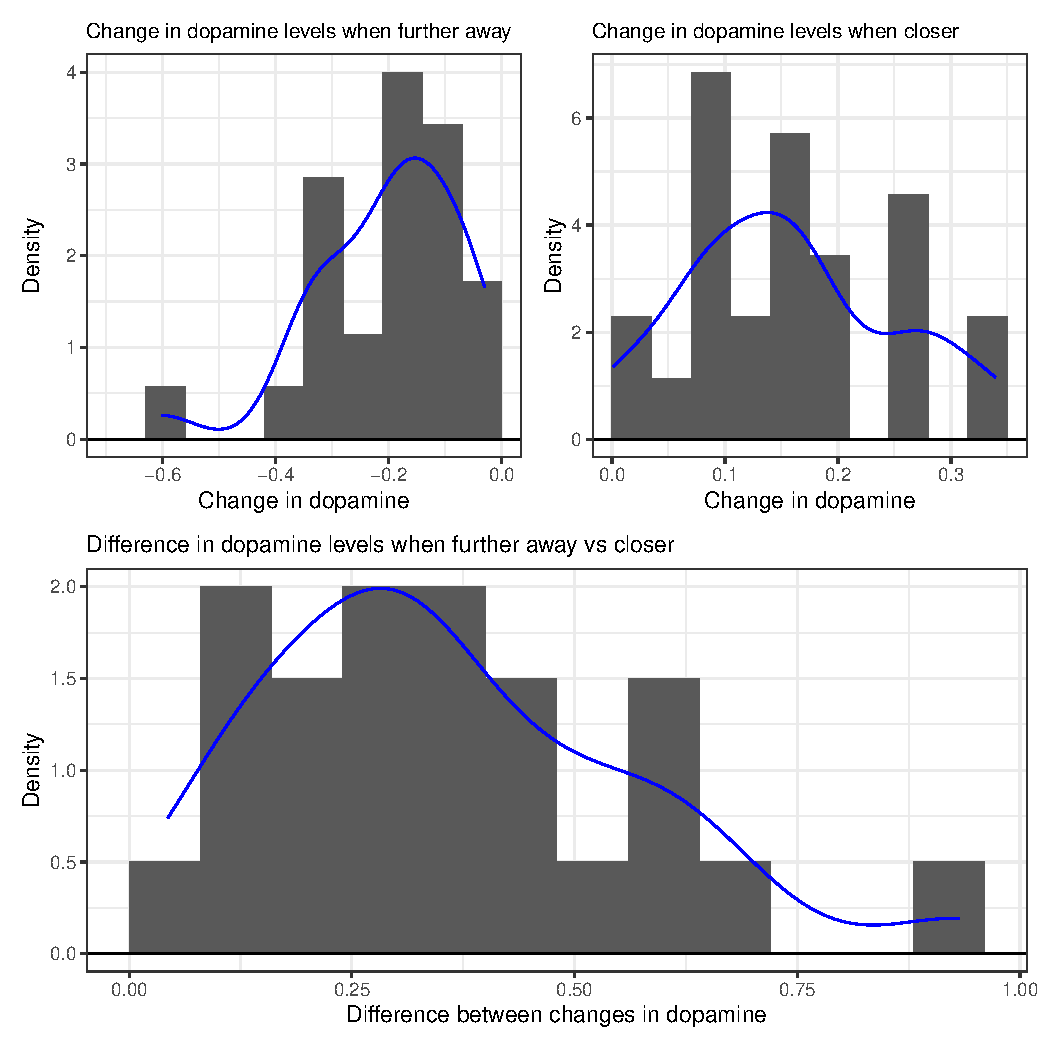
\includegraphics[width=\maxwidth]{figure/unnamed-chunk-4-1} 
\end{knitrout}
The data does suggest that dopamine levels decrease when young zebra finches sing further away from their adult song. Although some of the data is close to 0, every data point is negative, indicating dopamine decreased for every observation. We can say the opposite thing about young zebra finches when they sing closer to their adult song. Every observation is positive, meaning even if not always by much, they all increased in dopamine levels when singing close to their adult song.

When looking at the differences between the two sets of data, you can see there is quite a significant difference between changes in dopamine levels for the zebra finches, depending on whether they are closer or further away from their adult song. When doing closer - further, every observation is positive, meaning dopamine levels always change more positively when closer, than they do when further from their adult song. \\
Note that the plots don't follow a normal distribution very well, mainly due to the fact that we only have 25 observations for each data set.
  \item \textbf{Optional Challenge:} Can you reproduce Figure 2(g)?
  Note that the you can use \texttt{geom\_errorbar()} to plot
  the range created by adding the mean $\pm$ one standard deviation.
\end{enumerate}
%%%%%%%%%%%%%%%%%%%%%%%%%%%%%%%%%%%%%%%%%%%%%%%%%%%%%%%%%%%%%%%%%
% CONDUCT THE TESTS
%%%%%%%%%%%%%%%%%%%%%%%%%%%%%%%%%%%%%%%%%%%%%%%%%%%%%%%%%%%%%%%%%
\item Conduct the inferences they do in the paper. Make sure to report the results
a little more comprehensively -- that is your parenthetical should look something
like: ($t=23.99$, $p<0.0001$; $g=1.34$; 95\% CI: 4.43, 4.60).\\
\textbf{Note:} Your numbers may vary slightly as they performed some unclear
correction of their $p$-values. I'm waiting to hear back from them via email!
\begin{enumerate}
  \item ``The close responses differed significantly from 0 ($p=1.63 \times 10^{-8}$).''
\begin{knitrout}
\definecolor{shadecolor}{rgb}{0.969, 0.969, 0.969}\color{fgcolor}\begin{kframe}
\begin{alltt}
\hlkwd{library}\hldef{(effectsize)}
\hldef{closer.t.test} \hlkwb{=} \hlkwd{t.test}\hldef{(}\hlkwc{x}\hldef{=dopamine.data}\hlopt{$}\hldef{`Closer_vals`,}
                       \hlkwc{alternative} \hldef{=} \hlsng{"two.sided"}\hldef{,}
                       \hlkwc{mu} \hldef{=} \hlnum{0}\hldef{,}
                       \hlkwc{conf.level} \hldef{=} \hlnum{0.95}\hldef{)}
\hldef{g} \hlkwb{=} \hlkwd{hedges_g}\hldef{(}\hlkwc{x} \hldef{= dopamine.data}\hlopt{$}\hldef{`Closer_vals`,} \hlkwc{mu} \hldef{=} \hlnum{0}\hldef{,} \hlkwc{alternative} \hldef{=} \hlsng{"two.sided"}\hldef{)}
\end{alltt}
\end{kframe}
\end{knitrout}
t = 8.3024, p < 0.00000002, g = 1.61, 95\% CI: 0.1173875, 0.1950586 
  \item ``The far responses differed significantly from 0 ($p=5.17 \times 10^{-8}$).''
\begin{knitrout}
\definecolor{shadecolor}{rgb}{0.969, 0.969, 0.969}\color{fgcolor}\begin{kframe}
\begin{alltt}
\hldef{farther.t.test} \hlkwb{=} \hlkwd{t.test}\hldef{(}\hlkwc{x}\hldef{=dopamine.data}\hlopt{$}\hldef{`Farther_vals`,}
                       \hlkwc{alternative} \hldef{=} \hlsng{"two.sided"}\hldef{,}
                       \hlkwc{mu} \hldef{=} \hlnum{0}\hldef{,}
                       \hlkwc{conf.level} \hldef{=} \hlnum{0.95}\hldef{)}
\hldef{g} \hlkwb{=} \hlkwd{hedges_g}\hldef{(}\hlkwc{x} \hldef{= dopamine.data}\hlopt{$}\hldef{`Farther_vals`,} \hlkwc{mu} \hldef{=} \hlnum{0}\hldef{,} \hlkwc{alternative} \hldef{=} \hlsng{"two.sided"}\hldef{)}
\end{alltt}
\end{kframe}
\end{knitrout}
t = -7.778, p < 0.00000006, g = -1.51, 95\% CI: -0.2565176, -0.1489313 
  \item ``The difference between populations was significant ($p=1.04 \times10^{-8}$).''
\begin{knitrout}
\definecolor{shadecolor}{rgb}{0.969, 0.969, 0.969}\color{fgcolor}\begin{kframe}
\begin{alltt}
\hldef{differences.t.test} \hlkwb{=} \hlkwd{t.test}\hldef{(}\hlkwc{x}\hldef{=dopamine.data}\hlopt{$}\hldef{`difference`,}
                       \hlkwc{alternative} \hldef{=} \hlsng{"two.sided"}\hldef{,}
                       \hlkwc{mu} \hldef{=} \hlnum{0}\hldef{,}
                       \hlkwc{conf.level} \hldef{=} \hlnum{0.95}\hldef{)}
\hldef{g} \hlkwb{=} \hlkwd{hedges_g}\hldef{(}\hlkwc{x} \hldef{= dopamine.data}\hlopt{$}\hldef{`difference`,} \hlkwc{mu} \hldef{=} \hlnum{0}\hldef{,} \hlkwc{alternative} \hldef{=} \hlsng{"two.sided"}\hldef{)}
\end{alltt}
\end{kframe}
\end{knitrout}
t = 8.5109, p < 0.00000002, g = 1.65, 95\% CI: 0.2719028, 0.4459921


\end{enumerate}
%%%%%%%%%%%%%%%%%%%%%%%%%%%%%%%%%%%%%%%%%%%%%%%%%%%%%%%%%%%%%%%%%
% CONDUCT THE TESTS
%%%%%%%%%%%%%%%%%%%%%%%%%%%%%%%%%%%%%%%%%%%%%%%%%%%%%%%%%%%%%%%%%
\item Reverse engineer the hypothesis test plot from Lecture 20 to create accurate
hypothesis testing plots for each part of the previous question.
\begin{enumerate}
  \item Question 4, part(a).
  \item Question 4, part(b).
  \item Question 4, part(c).
\end{enumerate}
\end{enumerate}


\bibliography{bibliography}
\end{document}
